% !TEX program = xelatex
\documentclass[12pt]{article}
\usepackage[margin=1in]{geometry}
\usepackage{nopageno} % no page numbers
\usepackage{setspace} \doublespacing

\usepackage{graphicx}
\graphicspath{ {./graphics/} }
\usepackage[dvipsnames]{xcolor}
\definecolor{CrispBlue}{HTML}{0176AE}

\usepackage{fontspec}
\usepackage{tcolorbox}
\usepackage{etoolbox}
\BeforeBeginEnvironment{verbatim*}{\begin{tcolorbox}[colback=CrispBlue!5!white,colframe=CrispBlue!75!black]}%
\AfterEndEnvironment{verbatim*}{\end{tcolorbox}}%

\usepackage{hyperref}
\hypersetup{
    colorlinks,
    citecolor=black,
    filecolor=black,
    linkcolor=black,
    urlcolor=black
}

\renewcommand{\footnotesize}{\fontsize{8pt}{10pt}\selectfont}


\usepackage[labelfont={small,sc,bf},textfont={small,sc,bf}]{caption}
\setlength{\parindent}{24pt}
% \setlength{\parskip}{1em}

\usepackage{tocloft}
\renewcommand{\cftpartleader}{\cftdotfill{\cftdotsep}}
\renewcommand{\cftsecleader}{\cftdotfill{\cftdotsep}}

\usepackage[shortlabels]{enumitem}

\usepackage{lastpage}
\usepackage{fancyhdr}
\pagestyle{fancy}
\fancyhf{}
\renewcommand{\headrulewidth}{0pt}
\rfoot{Page \thepage\ of \pageref*{LastPage}}

\usepackage{amsmath,amsfonts,amssymb}
\usepackage{bm}
\usepackage{mathtools}

\renewcommand{\listfigurename}{List of Figures}

\begin{document}
\setmainfont{SF Pro Text}
\setsansfont{SF Pro Text}
\setmonofont{SF Mono}
\renewcommand{\familydefault}{\sfdefault}

\hypersetup{
    linkcolor=CrispBlue,
    urlcolor=CrispBlue,
    breaklinks=true
}

\noindent David Kirby\\
ECE 529: Introduction to Technical Cybersecurity\\
Spring, 2022
\begin{center}
    \large\bfseries Delivery System
\end{center}

% This assignment, part of the Reconnaissance and Vulnerability Identification\footnote{\href{https://learn.unm.edu/webapps/assignment/uploadAssignment?content_id=_7770481_1&course_id=_110809_1&user_id=_196414_1}{https://learn.unm.edu/webapps/assignment/uploadAssignment?content\_id=\_7770481\_1\&course\_id=\_110809\_1}} module, was designed to introduce students to the nmap scanning tool and to produce a detailed scan report for different hosts.

\textbf{Scenario I:}
We are attempting to deliver a rootkit into an IoT device in our professor's house. Our professor uses an older Windows installation for general work, email, and web browsing. He only uses a single subnet, some of which is wired, some of which is WiFi. We need to explore how to deliver the rootkit.

There are two possible attack vectors for this target. We could potentially use exploitkits to compromise the system via browser since we know that the professor uses his computer for web browsing. Additionally, we could attempt to penetrate the system using phishing. As Dr. Lamb mentioned in the lecture videos, phishing works all too often, and we know that he uses his network-connected computer for email as well, so this could give us a entryway to the IoT system.

In this case, our target is very specific, and this campaign would be categorized as spear-phishing. I do not want to be caught using my UNM email to phish Dr. Lamb, and the University of New Mexico marks all email received from outside its domain as [External]. This small but effective tactic can help to flag phishing campaigns; therefore, I will attempt to phish Professor Lamb using one of his other email accounts. While sending a reply to one of my emails, Dr. Lamb appears to have used the Gmail app for iPad. Opening the email with a text editor, we can analyze the email header as shown in Figure~\ref{fig:email}. We see that the Gmail app has unintentionally revealed his personal email, giving us our target. Using this email, we could tap into https://haveibeenpwned.com and determine the breaches in which this email has been exposed. This speaks to one of the dangerous trends mentioned in the lecture videos -- emails being used as usernames.
\begin{figure}[!ht]
    \centering
    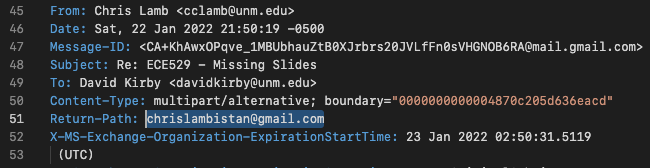
\includegraphics[width=\textwidth]{figure01.png}%\vspace{-1em}
    \caption{Email header exposing personal email.}
    \label{fig:email}
\end{figure}

Doing some reconnaissance, we see that Dr. Lamb has a Pinterest\footnote{\href{http://www.chrislambistan.com}{https://www.pinterest.com/chrislambistan/}} account, a Blogger account\footnote{\href{http://www.chrislambistan.com}{http://www.chrislambistan.com}}, and was active on the Ubiquiti\footnote{\href{https://community.ui.com/questions/Dest-Unreachable-Bad-Code-9-on-basic-config-on-ER-X/625315ac-bae4-42b9-ad83-6c716fd66ea7}{https://community.ui.com/questions/Dest-Unreachable-Bad-Code-9-on-basic-config-on-ER-X/625315ac-bae4-42b9-ad83-6c716fd66ea7}} community forums; the latter revealing some of the network equipment that Dr. Lamb is using in his home (see Figure~\ref{fig:ubiquiti}). This network equipment could be targeted for exploits\footnote{\href{https://nvd.nist.gov/vuln/search/results?form_type=Basic&results_type=overview&query=edgeos&search_type=all&isCpeNameSearch=false}{https://nvd.nist.gov/vuln/search/results?form\_type=Basic\&results\_type=overview\&query=edgeos\&search\_type=all-\&isCpeNameSearch=false}} and allow us to reach our end goal of delivering a rootkit to the Dr. Lamb's IoT device (and much more). All of this was discovered before even starting our spear-phishing campaign.
\vspace{-7em}
\begin{figure}[!ht]
    \centering
    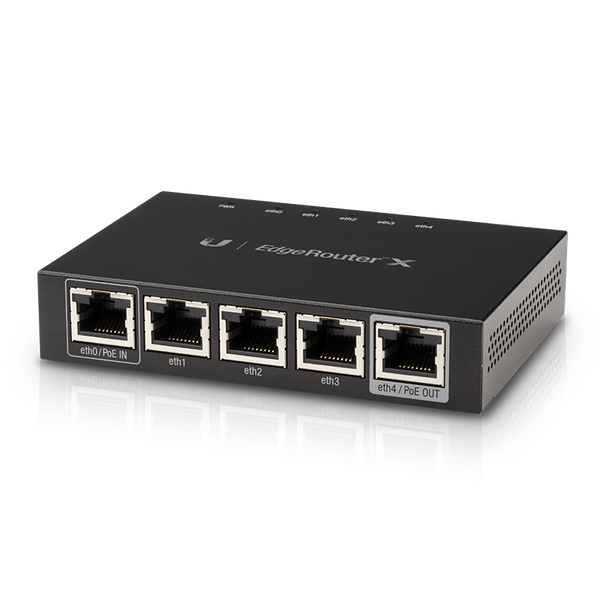
\includegraphics[width=0.7\textwidth]{figure02.png}\vspace{-4em}
    \caption[Network equipment discovered to be used by Dr. Lamb.]{Network equipment discovered to be used by Dr. Lamb.\protect\footnotemark}
    \label{fig:ubiquiti}
\end{figure}

\footnotetext{Image courtesy of Ubiquiti.}

Once we take what we have learned from our OSINT\footnote{\href{https://en.wikipedia.org/wiki/Open-source_intelligence}{https://en.wikipedia.org/wiki/Open-source\_intelligence}} tools, we can create a more targeted, and hopefully more successful phishing campaign. We could tailor emails so that Dr. Lamb would be more enticed to click on a link to a malicious site of our creation, exposing his system to our exploitkit and obtaining access to the network. We would use a two-payload design where the original payload would be delivered with the exploit, installed via his browser, and then downloads a secondary payload that has more functionality. From there, we show in Scenario II that it is trivial to pivot to the IoT device using its IP address and deliver a rootkit.

\textbf{Scenario II:}
We have an IoT device in a lab and we want to deliver a rootkit and crack contained passwords resident on the device. The device uses an old SSH daemon built around \texttt{libssh}. We will deliver the rootkit and exfiltrate the passwords.

As discussed in the lecture videos, \texttt{libssh} has an exploit revealed in 2018\footnote{\href{https://nvd.nist.gov/vuln/detail/CVE-2018-10933}{https://nvd.nist.gov/vuln/detail/CVE-2018-10933}} whereby the state machine that implements authentication had a flaw that would allow attackers to authenticate by transmitting a \texttt{SUCCESS} message instead of a \texttt{REQUEST}. Exploiting this flaw, we could circumvent authentication entirely by convincing the IoT device that we had already successfully authenticated. Once logged into the IoT device, we could explore the OS, most likely Linux-based, to retrieve the hashed passwords. We could look in the \texttt{/etc/shadow} or \texttt{/etc/password} folders depending on the age of the system, we could explore databases, or we could extract them from wire protocols.
Next, using password cracking tools as discussed in the video lectures, we can exfiltrate the plaintext passwords from the hashes. While exploring password cracking tools, I noticed that Cain and Abel is no longer available, even their website is defunct. Since I am using a Mac, I explored using two open source tools -- Search-That-Hash\footnote{\href{https://github.com/HashPals/Search-That-Hash}{https://github.com/HashPals/Search-That-Hash}} and Hashcat\footnote{\href{https://hashcat.net/hashcat/}{https://hashcat.net/hashcat/}} (both installed using brew, my favorite package manager for macOS). Search-That-Hash searches popular hash cracking sites and automatically inputs the hash(es) for cracking, but even more useful for us beginners, it has a tool to automatically identify the hash type (i.e. MD5, SHA family, etc.). Search-That-Hash can also run offline by piping the hashes to Hashcat. By implementing both of these tools, we could not only determine the type of hash used, but also crack and exfiltrate the passwords.

To mitigate these threats, my suggestion would be keeping operating systems, software, and IoT firmware regularly updated. I would also recommend Dr. Lamb set up a network firewall to block malicious actors. I personally also implement a DNS filter on my router that blocks trackers, malware, and advertisements network-wide. This prevents, for example, my smart thermostat from connecting to sites that I do not allow. This also gives me a log of traffic to my network and allows me to catch suspicious activity. Mitigating these attacks also requires due diligence when opening emails, links, and documents as we have seen that metadata can have a wealth of information with unforeseen consequences.



% \begin{tcolorbox}[colback=CrispBlue!5!white,colframe=CrispBlue!75!black,title=Output of \texttt{nmap -oN scanme-A.txt -A scanme.nmap.org}]\setstretch{1.25}

% \end{tcolorbox}



\end{document}